\documentclass{article}
\usepackage{graphicx} % Required for inserting images
\usepackage{braket}
\usepackage[margin=0.8in]{geometry}
\usepackage{amsmath}
\usepackage{amssymb}
\usepackage{amsthm}
\usepackage{enumitem}
\usepackage{mathrsfs}

\usepackage{tikz}
\usepackage{xcolor}
\usetikzlibrary{shapes.geometric, positioning}

\usepackage{biblatex}
\addbibresource{refs.bib}

\newcommand{\hilbert}{\mathcal{H}}
\newcommand{\Heff}{H_{\mathrm{eff}}}

\DeclareMathOperator{\trace}{Tr}
\DeclareMathOperator{\pfaff}{Pf}

\newtheorem{theorem}{Theorem}[section]

\newcommand{\hwnote}[1]{{\color{red}\textbf{HW:} #1}}

\title{A Summary of Kitaev and Laumann's\\\emph{Topological phases and quantum computation}}
\author{Heewon Lee}
\date{\today}

\begin{document}

\maketitle

\section{Introduction: The quest for protected qubits}
The motivation for investigating topological phases is given in the context of quantum computation.
While an ideal qubit is a system with exactly two degenerate states
(namely $\ket{0}$ and $\ket{1}$),
any physical system has a full spectrum of illegal states which,
if coupled to the logical states strongly, causes leakage into them,
manifesting as decoherence in the logical subspace.
Restricting one's interests only on the logical sector,
one defines an \emph{effective Hamiltonian} (Section~\ref{sec:feshbach}),
which is ideally $\Heff \propto 1$
(such that the time evolution of any ground state is simply obtaining a global phase).
The most elementary mechanism of protecting this degeneracy is
with a symmetry respected by the Hamiltonian such that $\ket{0}$ and $\ket{1}$
are in the same irreducible sector.
While any non-Abelian symmetry suffices (Section~\ref{sec:symmetry}), they are easily broken by stray fields and such.
Thus, one tries to find \emph{topological phases}
such that ground state degeneracy is topologically protected
and the spectrum is gapped.

\subsection{Feshbach projection}\label{sec:feshbach}
Suppose the Hilbert space can be decomposed into $\hilbert = \hilbert_P \oplus \hilbert_Q$,
with respective projection operators $P$ and $Q$.
Completeness requires $P + Q = 1$.
We wish to find an effective Hamiltonian $\Heff$ on $\hilbert_P$ such that
\[
    i\hbar\frac{\partial}{\partial t} P \ket{\psi} = \Heff P\ket{\psi}.
\]

Take an energy eigenstate $\ket{\psi}$ of the full system with energy $E$.
Let $\ket{\psi_P} := P \ket{\psi}$ and $\ket{\psi_Q} := Q\ket{\psi}$,
such that $\ket{\psi} = \ket{\psi_P} + \ket{\psi_Q}$.
Then, from $H\ket{\psi} = E\ket{\psi}$, one finds the following two relations:
\[
    E\ket{\psi_P} = PHP\ket{\psi_P} + PHQ\ket{\psi_Q},
\]
\[
    E\ket{\psi_Q} = QHP\ket{\psi_P} + QHQ\ket{\psi_Q}.
\]
Solving for $\ket{\psi_Q}$ from the second equation and substituting it into the first, one finds:
\[
    E\ket{\psi_P} = \left( PHP + PHQ \left(E-QHQ\right)^{-1} QHP \right) \ket{\psi_P},
\]
thus the right-hand side acting as the effective Hamiltonian.

Additionally, suppose $H = H_0 + V$ with $H_0$ solvable
with no coupling between $\hilbert_P$ and $\hilbert_Q$ (i.e., $PH_0Q = QH_0P=0$),
and $V$ tiny (in the perturbative sense).
In this case, using the identity (where $A$ is invertible)\footnote{%
    The series expansion holds for $\lVert A^{-1} B \rVert < 1$.
}
\[
    \left(A-B\right)^{-1} = \left(I - A^{-1}B\right)^{-1} \cdot A^{-1}
    = \sum_{n=0}^\infty \left(A^{-1}B\right)^n A^{-1},
\]
we obtain the final expression
\[
    \Heff = PHP + PVQ (E-QH_0Q)^{-1} QVP + PVQ (E-QH_0Q)^{-1} QVQ (E-QH_0Q)^{-1} QVP + \cdots.
\]
While the equation is exact when $E$ is a true eigenenergy of the original Hamiltonian,
meaning solving the self-consistent equation $\mathrm{det} \left( E - \Heff(E)\right) = 0$
yields the exact energies of the full system,
it is often numerically approximated, e.g., with an iterative scheme.
Moreover, if the coupling is sufficiently weaker than the spectrum gap
(i.e., $\lVert V \rVert \ll \Delta$),
one can neglect the $E$-dependency of the right-hand side to get
\[
    \Heff \approx PHP - PVQ (QH_0Q)^{-1} QVP  + PVQ(QH_0Q)^{-1}QVQ(QH_0Q)^{-1}QVP + \cdots.
\]

\subsection{Symmetry-based degeneracy}\label{sec:symmetry}
Suppose $G$ is a group with a unitary representation $U: G \to U(\hilbert)$.
Now assume that the Hamiltonian $H$ respects this symmetry:
$\forall g \in G.\; U(g)^\dagger H U(g) = H$.
This implies that $H$ commutes with every $U(g)$.
Then, by Schur's lemma, $H$ restricted to any irreducible subspace of $\hilbert$
must be a multiple of the identity.
Therefore, if the ground state manifold is contained within an irreducible subspace of $\hilbert$,
then $G$ enforces that the Hamiltonian on the ground state manifold is trivial.

If $G$ is Abelian, this argument cannot protect any degeneracy.
Suppose $U(g_1)U(g_2) = U(g_2)U(g_1)$ for any $g_1, g_2 \in G$.
Then, a given $U(g)$ commutes with every other $U(g')$.
Thus, again by Schur's lemma, $U(g) \propto 1$ on any irreducible subspace,
but since every one-dimensional subspace is invariant under scalar multiplication,
any irreducible subspace must be one-dimensional.
Therefore, Abelian symmetries fail to protect any degeneracy between states.

% =========================================
\section{Topological phenomena in 1D: boundary modes in the Majorana chain}
The following three one-dimensional models are considered in this section.
They will be found to represent equivalent physics, with suitable transformations between them.
\hwnote{Why are these interesting models to study?
The Kitaev chain was first motivated as an unrealistic example demonstrating unpaired Majoranas.~\cite{kitaev2001}
}
\begin{enumerate}
    \item \emph{XY model}:
        Spin-$\frac{1}{2}$ model with nearest-neighbor (anti)aligning interaction in the $x, y$ directions
        and external magnetic field in the $z$ direction.
        \[
            H_S = -J_x\sum_{j=1}^{N-1} \sigma_j^x \sigma_{j+1}^x
                  -J_y\sum_{j=1}^{N-1} \sigma_j^y \sigma_{j+1}^y
                  - h_z \sum_{j=1}^N \sigma_j^z
        \]

    \item \emph{Spin-polarized superconductor} (SPSC):
        Fermionic system with nearest-neighbor hopping, pair generation and annihilation, and chemical potential.\footnote{\label{foot:parity-super}%
        This model can be motivated as follows:
        The \emph{fermionic parity superselection rule} dictates that every physical observable of fermions must preserve parity,
        that is, cannot be an odd polynomial of fermionic fields.
        This stems from relativistic field-theoretic considerations,
        wherein spacelike-separated observables must commute to prevent faster-than-light communication.
        The terms appearing in the Hamiltonian are precisely
        the quadratic terms permitted by the superselection rule,
        with the pair generation and annihilation terms preserving parity but breaking number conservation.
        Additional constraints such as locality and dimensionality yield this Hamiltonian.
        }
        \hwnote{In what sense is this a superconductor? Can I calculate the conductance, say with NEGF?}
        \[
            H_F = \sum_{j=1}^{N-1} \left(
                -w\left(a_j^\dagger a_{j+1} + a_{j+1}^\dagger a_j \right)
                +\Delta a_j a_{j+1} + \Delta^* a_{j+1}^\dagger a_j^\dagger
            \right)
            -\mu \sum_{j=1}^N \left( a_j^\dagger a_j - \frac{1}{2} \right)
        \]

    \item \emph{Majorana system} with pairwise nearest-neighbor interaction:
        (See Figure~\ref{fig:majorana} for the coupling connectivity.)
        \[
            H_{maj} = \frac{i}{2} \left(
                \alpha \sum_{j=1}^N c_{2j-1}c_{2j}
                + \beta \sum_{j=1}^{N-1} c_{2j}c_{2j+1}
                + \gamma \sum_{j=1}^{N-1} c_{2j-1}c_{2j+2}
            \right)
        \]
\end{enumerate}

\begin{figure}[ht]
    \centering
    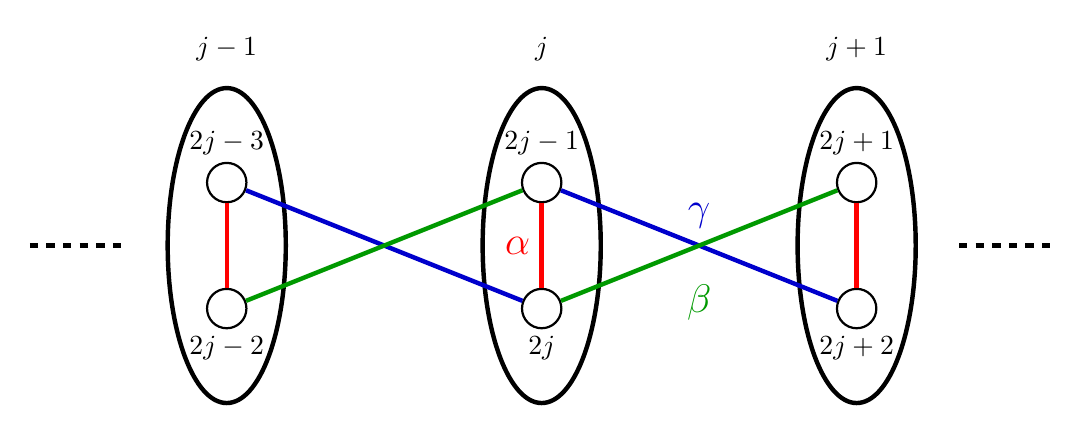
\begin{tikzpicture}[
        >=stealth,
        thick,
        % Style for the large vertical ellipses
        bigellipse/.style={ellipse, draw=black, ultra thick, minimum width=1.5cm, minimum height=4cm},
        % Style for the inner circles
        smallcircle/.style={circle, draw=black, thick, minimum size=0.5cm, inner sep=0pt}
    ]
    
        % --- Nodes for 2j-1 ---
        \node[bigellipse] (E1) at (0,0) {};
        \node at (0, 2.5) {$j-1$};
        \node[smallcircle] (A1) at (0, 0.8) {};
        \node at (0, 1.3) {$2j-3$};
        \node[smallcircle] (B1) at (0, -0.8) {};
        \node at (0, -1.3) {$2j-2$};
    
        % --- Nodes for 2j ---
        \node[bigellipse] (E2) at (4,0) {};
        \node at (4, 2.5) {$j$};
        \node[smallcircle] (A2) at (4, 0.8) {};
        \node at (4, 1.3) {$2j-1$};
        \node[smallcircle] (B2) at (4, -0.8) {};
        \node at (4, -1.3) {$2j$};
    
        % --- Nodes for 2j+1 ---
        \node[bigellipse] (E3) at (8,0) {};
        \node at (8, 2.5) {$j+1$};
        \node[smallcircle] (A3) at (8, 0.8) {};
        \node at (8, 1.3) {$2j+1$};
        \node[smallcircle] (B3) at (8, -0.8) {};
        \node at (8, -1.3) {$2j+2$};
    
        % --- Dashed lines at the ends ---
        \draw[dashed, ultra thick] (-2.5, 0) -- (-1.3, 0);
        \draw[dashed, ultra thick] (9.3, 0) -- (10.5, 0);
    
        % --- Red Vertical Lines & Label ---
        \draw[red, ultra thick] (A1) -- (B1);
        \draw[red, ultra thick] (A2) -- (B2) node[midway, left] {\Large $\alpha$};
        \draw[red, ultra thick] (A3) -- (B3);
    
        % --- Blue Lines & Label ---
        \draw[blue!80!black, ultra thick] (A1) -- (B2);
        \draw[blue!80!black, ultra thick] (A2) -- (B3) 
            node[midway, above=2pt, blue!80!black] {\Large $\gamma$};
    
        % --- Green Lines & Label ---
        \draw[green!60!black, ultra thick] (B1) -- (A2);
        \draw[green!60!black, ultra thick] (B2) -- (A3) 
            node[midway, below=10pt, green!60!black] {\Large $\beta $};
    
    \end{tikzpicture}
    \caption{Connectivity diagram for the Majorana system}
    \label{fig:majorana}
\end{figure}
A common special case is observed for the three representations:
\begin{enumerate}
    \item \emph{Transverse-field Ising model} (TFIM): XY model with $J_y = 0$
    \item SPSC with $\Delta = \Delta^* = w$
    \item Majorana system with $\gamma = 0$
\end{enumerate}

Also, the system posseses a $\mathbb{Z}_2$ symmetry with respective transformations:
\[
    P_S = \prod_{j=1}^N \sigma_j^z,\quad
    P_F = \prod_{j=1}^N \left( 1 - 2a_j^\dagger a_j \right),\quad
    P_{maj} = \prod_{j=1}^N \left( -ic_{2j-1}c_{2j} \right).
\]

\subsection{Nature of topological degeneracy (spin language)}\label{sec:ising}
Consider the Ising model with $h_z$ small enough such that perturbation theory applies.
The two ground states are given by $\ket{\rightarrow \rightarrow \cdots \rightarrow}$
and $\ket{\leftarrow\leftarrow \cdots \leftarrow}$.
(In this subsection, all spin language supposes the $x$ basis.)
A state with any other spin configuration is considered illegal,
and the magnetic field term flips a single spin;
hence, any two states differing by one spin flip are coupled.
Thus, using the Feshbach expansion, the tunneling amplitude becomes:
\[
    t := \braket{\left\{\leftarrow\right\} | \Heff | \left\{\rightarrow\right\}}
    \approx \sum_{l} (-1)^{\lVert l \rVert} \frac{h_z^{\lVert l\rVert}}{\prod_{\alpha\in l} E_\alpha},
\]
where $l$ ranges over all paths from $\ket{\rightarrow \rightarrow \cdots \rightarrow}$
to $\ket{\leftarrow\leftarrow \cdots \leftarrow}$,
and $\alpha$ over states passed through $l$ except the above two.
The most dominant term comes from the path of a single domain wall traversing:
\[
    \ket{\rightarrow\rightarrow\cdots\rightarrow}
    \longrightarrow \ket{\leftarrow:\rightarrow\cdots\rightarrow}
    \longrightarrow \ket{\leftarrow\leftarrow:\cdots\rightarrow}
    \longrightarrow \cdots
    \longrightarrow \ket{\leftarrow\leftarrow\cdots\leftarrow}.
\]
With each $E_\alpha$ equal and of order $J_x$, one finds that $t \sim h_z^N / J_x^{N-1}$, or
\[
    t \sim J_xe^{-N/\xi}\quad \text{ with }\quad \xi^{-1} = \ln\left( \frac{J_x}{h_z} \right).
\]
Thus, the effective Hamiltonian is given by
\[
    \Heff = \begin{pmatrix}
        0 & -t \\ -t & 0
    \end{pmatrix},
\]
exponentially decaying with the length of the chain;
particularly, the degeneracy is recovered in the thermodynamic limit.

\subsection{Reduction of TFIM to SPSC by the Jordan-Wigner transformation}
For a single site, spin-$\frac{1}{2}$ particle and a spinless fermion can be readily identified:
\[
    \ket{\uparrow} \leftrightarrow \ket{0},\quad
    \ket{\downarrow} \leftrightarrow \ket{1},\quad
    \frac{\sigma^x \pm i \sigma^y}{2} \leftrightarrow \begin{Bmatrix} a \\ a^\dagger \end{Bmatrix}.
\]
However, once multiple sites are introduced, the fermionic exchange statistics must be considered.
For a 1D chain with open boundaries, this can be done by the \emph{Jordan-Wigner transformation}:
\[
    \left( \prod_{i<j} \sigma_i^z \right) \left( \frac{\sigma_j^x \pm i\sigma_j^y}{2} \right)
    \leftrightarrow \begin{Bmatrix} a \\ a^\dagger \end{Bmatrix},
\]
which satisfies the anticommutation relation $\left\{a_i, a_j^\dagger\right\} = \delta_{ij}$
and implies $\sigma_j^z = 1 - 2a_j^\dagger a_j$.
The open boundary condition is crucial for $i<j$ to be well-defined,
meaning the Jordan-Wigner string could terminate without introducing
another boundary term.

We now drop the $\leftrightarrow$ symbol and just use equality.
Routine calculations yield:
\begin{align*}
    \sigma_j^z &= 1 - 2a_j^\dagger a_j \\
    \sigma_j^x \sigma_{j+1}^x &= \left(a_j^\dagger a_{j+1} + a_{j+1}^\dagger a_j\right)
                               - \left(a_j a_{j+1} + a_{j+1}^\dagger a_j^\dagger\right) \\
    \sigma_j^y \sigma_{j+1}^y &= \left(a_j^\dagger a_{j+1} + a_{j+1}^\dagger a_j\right)
                               + \left(a_j a_{j+1} + a_{j+1}^\dagger a_j^\dagger\right)
\end{align*}
Thus, the XY model and SPSC chain are identified via
\begin{align*}
    H_S
    &= -J_x\sum_{j=1}^{N-1} \sigma_j^x \sigma_{j+1}^x
       -J_y\sum_{j=1}^{N-1} \sigma_j^y \sigma_{j+1}^y
       -h_z \sum_{j=1}^N \sigma_j^z \\
    &= \sum_{j=1}^{N-1} \left(
        -\left( J_x + J_y \right) \left( a_j^\dagger a_{j+1} + a_{j+1}^\dagger a_j \right)
        +\left( J_x - J_y \right) \left( a_ja_{j+1} + a_{j+1}^\dagger a_j^\dagger \right)
    \right) + 2h_z \sum_{j=1}^N \left( a_j^\dagger a_j - \frac{1}{2} \right)
\end{align*}
\[
    \therefore w = J_x + J_y,\quad
    \Delta = \Delta^* = J_x - J_y,\quad
    \mu = -2h_z.
\]
The $\mathbb{Z}_2$ operators $P_S$ and $P_F$
and the conditions $J_y = 0 \iff \Delta = \Delta^* = w$ are identified.
Note that $\Delta \in \mathbb{R}$ is not a physical constraint on the model,
as the phase $\Delta = |\Delta| e^{i\alpha}$ can be absorbed by a mere basis redefinition
$a_j \mapsto a_j e^{i\alpha/2}$.

\subsection{Majorana operators}
The \emph{Majorana fermions} are fermions that are their own antiparticles.
While first formulated in the context of field theory and applied to neutrinos,
the Majorana operators are useful in many fields, not least because the creation/annihilation operators
are Hermitian and square to one.
Thus, one defines:
\[
    c_{2j-1} := a_j + a_j^\dagger,\quad
    c_{2j} := i\left(a_j^\dagger - a_j\right).
\]
The Majorana operators satisfy the anticommutation relation $\left\{c_j, c_k\right\} = 2\delta_{jk}$.

Again, routine calculations allow us to identify the SPSC chain and the quadratic Majorana system:
\begin{align*}
    a_j^\dagger a_j &= \frac{1}{2}\left(1 + ic_{2j-1}c_{2j}\right)\\
    a_j^\dagger a_{j+1} + a_{j+1}^\dagger a_j &= \frac{i}{2}\left(-c_{2j}c_{2j+1} + c_{2j-1}c_{2j+2}\right) \\
    a_j a_{j+1} + a_{j+1}^\dagger a_j^\dagger &= \frac{i}{2}\left(c_{2j}c_{2j+1} + c_{2j-1}c_{2j+2}\right)
\end{align*}
\begin{align*}
    \implies H_F
    &= \sum_{j=1}^{N-1} \left(
            -w\left(a_j^\dagger a_{j+1} + a_{j+1}^\dagger a_j \right)
            +\Delta \left(a_j a_{j+1} + a_{j+1}^\dagger a_j^\dagger \right)
        \right)
        -\mu \sum_{j=1}^N \left( a_j^\dagger a_j - \frac{1}{2} \right) \\
    &= \frac{i}{2} \left(
        -\mu \sum_{j=1}^N c_{2j-1} c_{2j}
        + (w+\Delta) \sum_{j=1}^{N-1} c_{2j} c_{2j+1}
        + (\Delta - w) \sum_{j=1}^{N-1} c_{2j-1} c_{2j+2}
    \right)
\end{align*}
\[
    \therefore \alpha = -\mu,\quad
    \beta = w + \Delta,\quad
    \gamma = \Delta - w
\]
(Caution: The paper itself has a typo, the last correspondence differing by a factor of two.)
Thus, the three models can be identified, with the $\mathbb{Z}_2$ operators $P_S, P_F, P_{maj}$ all equivalent.
The special case is given by $\Delta = w \iff \gamma = 0$ as expected.

Additionally, $\gamma$ cannot be eliminated by a mere local $O(2)$ redefinition:
\[
    \begin{pmatrix}
        b_{2j-1} & b_{2j}
    \end{pmatrix} = \begin{pmatrix}
        c_{2j-1} & c_{2j}
    \end{pmatrix} \begin{pmatrix}
        \cos\theta & \sin\theta \\ \mp\sin\theta & \pm\cos\theta
    \end{pmatrix}.
\]
In the Majorana formulation, this can be seen because there are four possible interactions
($b_{2j-1}b_{2j+1}$, $b_{2j-1}b_{2j+2}$, $b_{2j}b_{2j+1}$, $b_{2j}b_{2j+2}$),
meaning a single variable $\theta$ is insufficient in general to eliminate three of them.
Thus, the point $\Delta = w$ is a genuine property of the Hamiltonian
rather than a basis choice.

\subsection{General properties of quadratic fermionic Hamiltonians}\label{sec:quadratic}
Notice how every term in the previous Hamiltonian was of the form $ic_jc_k$.
In a sense, this is the only possible two-Majorana interaction, compared to the four two-Dirac interactions
($a_j a_k, a_j a_k^\dagger, \dots$).
Thus, rather than studying only the Kitaev chain,
we instead investigate the structure of general quadratic Hamiltonians,
of which the Kitaev chain is a particular example:
\[
    H(M) = \frac{i}{4} \sum_{jk} M_{jk} c_j c_k.
\]
Notice that it is linear in $M$, so one may consider the decomposition $M = S + A$,
with $S^\dagger = S$ and $A^\dagger = -A$, and write $H(M) = H(S) + H(A)$.
The former results in a mere constant shift of energy and can be neglected:
\[
    H(S) = \frac{i}{4} \sum_{jk} S_{jk} c_j c_k = \frac{i}{8}\sum_{jk} S_{jk} \left\{c_j, c_k\right\}
    = \frac{i}{4} \trace S = \mathrm{const.}
\]
Then, the Hermicity forces $A$ to be real:
\[
    H(A)^\dagger = -\frac{i}{4}\sum_{jk} A_{jk}^* c_k c_j = \frac{i}{4} \sum_{jk} A_{jk}^* c_j c_k = H(A)
    \implies A_{jk} = A_{jk}^* \implies A_{jk} \in \mathbb{R}.
\]
Therefore, without loss of generality, we only consider $A \in \mathfrak{so}(2N)$,
or real skew-symmetric matrices.


The coefficient $\frac{i}{4}$ is chosen such that
the mapping $-iH: \mathfrak{so}(2N) \rightarrow \mathfrak{spin}(2N)$ is a Lie algebra homomorphism:
\begin{align*}
    [-iH(A), -iH(B)]
    &= \frac{1}{16} \sum_{jklm} A_{jk} B_{lm} [c_j c_k, c_l c_m] \\
    &= \frac{1}{16} \sum_{jklm} A_{jk} B_{lm} \left(
        c_j \left\{c_k, c_l\right\} c_m
        - \left\{c_j, c_l\right\} c_k c_m
        + c_l c_j \left\{c_k, c_m\right\}
        - c_j \left\{c_j, c_m\right\} c_k
    \right) \\
    &= \frac{1}{4} \sum_{ijk} \left(A_{ik} B_{kj} - B_{ik} A_{kj}\right) c_i c_j \\
    &= -iH([A, B]).
\end{align*}
Therefore, the classification of quadratic Hamiltonians can be reduced to the algebraic structure of $\mathfrak{so}(2N)$.
\hwnote{What are the spin group and algebra? What do their algebraic structures inform us about Majorana physics?}

A real skew-symmetric matrix $A$ has purely imaginary eigenvalues with complex conjugate pairs,
so it may be block-diagonalized as:
\[
    A = Q \begin{pmatrix}
        0           & \epsilon_1 &             &            &        \\
        -\epsilon_1 & 0          &             &            &        \\
                    &            & 0           & \epsilon_2 &        \\
                    &            & -\epsilon_2 & 0          &        \\ 
                    &            &             &            & \ddots
    \end{pmatrix} Q^t \quad
    (Q \in O(2N),\; \epsilon_j \geq 0)
\]
Notice how, considering $\vec{c}$ to be a row vector and $\vec{b} := \vec{c}Q$, one finds:
\[
    H(A) = \frac{i}{4} \vec{c} A \vec{c}^t
    = \frac{i}{4} \vec{b} \begin{pmatrix}
        0           & \epsilon_1 &             &            &        \\
        -\epsilon_1 & 0          &             &            &        \\
                    &            & 0           & \epsilon_2 &        \\
                    &            & -\epsilon_2 & 0          &        \\ 
                    &            &             &            & \ddots
    \end{pmatrix} \vec{b}^t,
\]
meaning each pair $b_{2j-1}, b_{2j}$ defines an independent sector with eigenenergies $\pm \frac{\epsilon_j}{2}$.
In particular, if $\epsilon_j = 0$, then the sector is twofold degenerate and decoupled from the other states.

For the Majorana model of our interest, the $A$ matrix is given in the heptadiagonal form:
\[
    A = \begin{pmatrix}
        0       & \alpha & 0       & \gamma  &         &        &        \\
        -\alpha & 0      & \beta   & 0       & 0       &        &        \\
        0       & -\beta & 0       & \alpha  & 0       & \gamma &        \\
        -\gamma & 0      & -\alpha & 0       & \beta   & 0      & \ddots \\
                & 0      & 0       & -\beta  & 0       & \alpha & \ddots \\
                &        & -\gamma & 0       & -\alpha & 0      & \ddots \\
                &        &         & \ddots  & \ddots  & \ddots & \ddots
    \end{pmatrix}.
\]
Notice that the nonzero entries are placed in a checkerboard fashion: odd rows on even columns, and vice versa.
In principle, for a finite chain, one can diagonalize this finite matrix to find the exact eigenstates.

To find the zero modes, one solves the system of equations $\vec{u}A = 0$, or
\[
    \begin{cases}
        -\alpha u_2 - \gamma u_4 = 0 \\
        \alpha u_1 - \beta u_3 = 0 \\
        \quad\vdots \\
        \beta u_{2j} - \alpha u_{2j+2} - \gamma u_{2j+4} = 0 \\
        \gamma u_{2j-1} + \alpha u_{2j+1} - \beta u_{2j+3} = 0 \\
        \quad\vdots \\
        \beta u_{2N-2} - \alpha u_{2N} = 0 \\
        \gamma u_{2N-3} + \alpha u_{2N-1} = 0
    \end{cases}
\]
Because of the aforementioned checkerboard fashion, this system is bipartite,
that is, $\left\{u_{2j}\right\}$ and $\left\{u_{2j-1}\right\}$ are independent of each other.

In general, this equation does not have any nontrivial solutions.
To show that this is the case, one can recursively find the \emph{Pfaffian} of $A$,
whose square is the determinant.
\[
    p_n := \pfaff \begin{pmatrix}
        0       & \alpha & 0       & \gamma  &         &        &        \\
        -\alpha & 0      & \beta   & 0       & 0       &        &        \\
        0       & -\beta & 0       & \alpha  & 0       & \gamma &        \\
        -\gamma & 0      & -\alpha & 0       & \beta   & 0      & \ddots \\
                & 0      & 0       & -\beta  & 0       & \alpha & \ddots \\
                &        & -\gamma & 0       & -\alpha & 0      & \ddots \\
                &        &         & \ddots  & \ddots  & \ddots & \ddots
    \end{pmatrix}
    = (\text{Cofactor expansion})
    = \alpha p_{n-1} + \beta\gamma p_{n-2},\quad
    p_0 = 1,\quad
    p_1 = \alpha
\]
One immediately finds several parameter values at which the Pfaffian vanishes,
namely if $\alpha = \gamma = 0$ or if $\alpha = 0$ and $N$ is odd.
\hwnote{Why would the parity of $N$ matter? Number of Majorana operators in each disconnected chain? Parity superselection?}
However, fine tuning of the parameters is necessary to obtain exact zero eigenenergies for a given $N$.

We thus want to investigate whether the model possesses near-zero modes or not.
To that end, we approximate them as the exact zero modes found in semi-infinite chains,
where only one boundary is considered.
Take the left boundary mode as example.
To compact the notation, we utilize \emph{transfer matrices}:
\[
    \begin{pmatrix}
        u_{2j+3} \\ u_{2j+1}
    \end{pmatrix} = \begin{pmatrix}
        \frac{\alpha}{\beta} & \frac{\gamma}{\beta} \\ 1 & 0
    \end{pmatrix} \begin{pmatrix}
        u_{2j+1} \\ u_{2j-1}
    \end{pmatrix},\quad
    \alpha u_1 - \beta u_3 = 0,
\]
\[
    \begin{pmatrix}
        u_{2j+4} \\ u_{2j+2}
    \end{pmatrix} = \begin{pmatrix}
        -\frac{\alpha}{\gamma} & \frac{\beta}{\gamma} \\ 1 & 0
    \end{pmatrix} \begin{pmatrix}
        u_{2j+2} \\ u_{2j}
    \end{pmatrix},\quad
    -\alpha u_2 - \gamma u_4 = 0.
\]
This yields the general formula:
\[
    \begin{pmatrix}
        u_{2j+1} \\ u_{2j-1}
    \end{pmatrix} = \begin{pmatrix}
        \frac{\alpha}{\beta} & \frac{\gamma}{\beta} \\ 1 & 0
    \end{pmatrix}^{j-1} \begin{pmatrix}
        \frac{\alpha}{\beta} \\ 1
    \end{pmatrix}
    \implies
    u_{2j-1} = \frac{\beta}{\sqrt{\alpha^2 + 4\beta\gamma}}\left(
        \left(\frac{\alpha+\sqrt{\alpha^2+4\beta\gamma}}{2\beta}\right)^j
        - \left(\frac{\alpha-\sqrt{\alpha^2+4\beta\gamma}}{2\beta}\right)^j
    \right),
\]
\[
    \begin{pmatrix}
        u_{2j+2} \\ u_{2j}
    \end{pmatrix} = \begin{pmatrix}
        -\frac{\alpha}{\gamma} & \frac{\beta}{\gamma} \\ 1 & 0
    \end{pmatrix}^{j-1} \begin{pmatrix}
        -\frac{\alpha}{\gamma} \\ 1
    \end{pmatrix}
    \implies
    u_{2j} = \frac{\gamma}{\sqrt{\alpha^2+4\beta\gamma}} \left(
        \left(\frac{-\alpha+\sqrt{\alpha^2+4\beta\gamma}}{2\gamma}\right)^j
        - \left(\frac{-\alpha-\sqrt{\alpha^2+4\beta\gamma}}{2\gamma}\right)^j
    \right).
\]
For these states to be normalizable, or at least relevant in the thermodynamic limit,
the coefficients must decay as $j$ increases, evidently exponentially.
However, notice that the product of all four bases is equal to one:
\[
    \left(\frac{\alpha+\sqrt{\alpha^2+4\beta\gamma}}{2\beta}\right)
    \left(\frac{\alpha-\sqrt{\alpha^2+4\beta\gamma}}{2\beta}\right)
    = -\frac{\gamma}{\beta},\quad
    \left(\frac{-\alpha+\sqrt{\alpha^2+4\beta\gamma}}{2\gamma}\right)
    \left(\frac{-\alpha-\sqrt{\alpha^2+4\beta\gamma}}{2\gamma}\right)
    = -\frac{\beta}{\gamma}.
\]
Thus, it is impossible that both $\left\{u_{2j-1}\right\}$ and $\left\{u_{2j}\right\}$ are square-normalizable,
meaning at most only one left near-zero mode could exist, for a given set of parameters $(\alpha, \beta, \gamma)$.
The same arguments apply for the right boundary mode once we replace $u_{j}$ with $u_{2N-j}$.\footnote{%
The condition $\alpha^2+4\beta\gamma = \mu^2 + 4\left(\Delta^2 - w^2\right) = 0$ is problematic,
in which case the geometric sequences are replaced with ones of the form $(A+Bj)r^j$.
}\footnote{%
After completing the derivation presented here, I became aware of \textcite{hedge_vishveshwara},
who analyze the Kitaev chain using the transfer-matrix formalism
and obtain analogous expressions for the boundary Majorana wavefunctions.
They further investigate several physical consequences
of the oscillatory regime ($\alpha^2+4\beta\gamma<0$), including:
\begin{enumerate}
    \item the exponentially small energy splitting acquires an oscillatory form,
    \[
        \epsilon \sim e^{-N/\xi}\cos(kN+\phi);
    \]
    \item the discrete parameter values at which a finite chain supports exact
    zero modes correspond to zeros of the oscillatory overlap;
    \item the ground-state fermion parity switches whenever the sign of the
    oscillatory splitting changes.
\end{enumerate}
}
The conditions for which a boundary mode exists has been numerically graphed in Figure~\ref{fig:phase},
and are algebraically verified in section~\ref{sec:phase}.
We thus find the following phase diagram:
\[
    \begin{cases}
        |\mu| < 2|w| & (\text{Topological phase; two boundary Majorana modes}) \\
        |\mu| > 2|w| & (\text{Trivial phase; no Majorana zero modes})
    \end{cases}
\]
See also section~\ref{sec:invar} for defining a topological invariant distinguishing these phases.

\begin{figure}[ht]
    \centering
    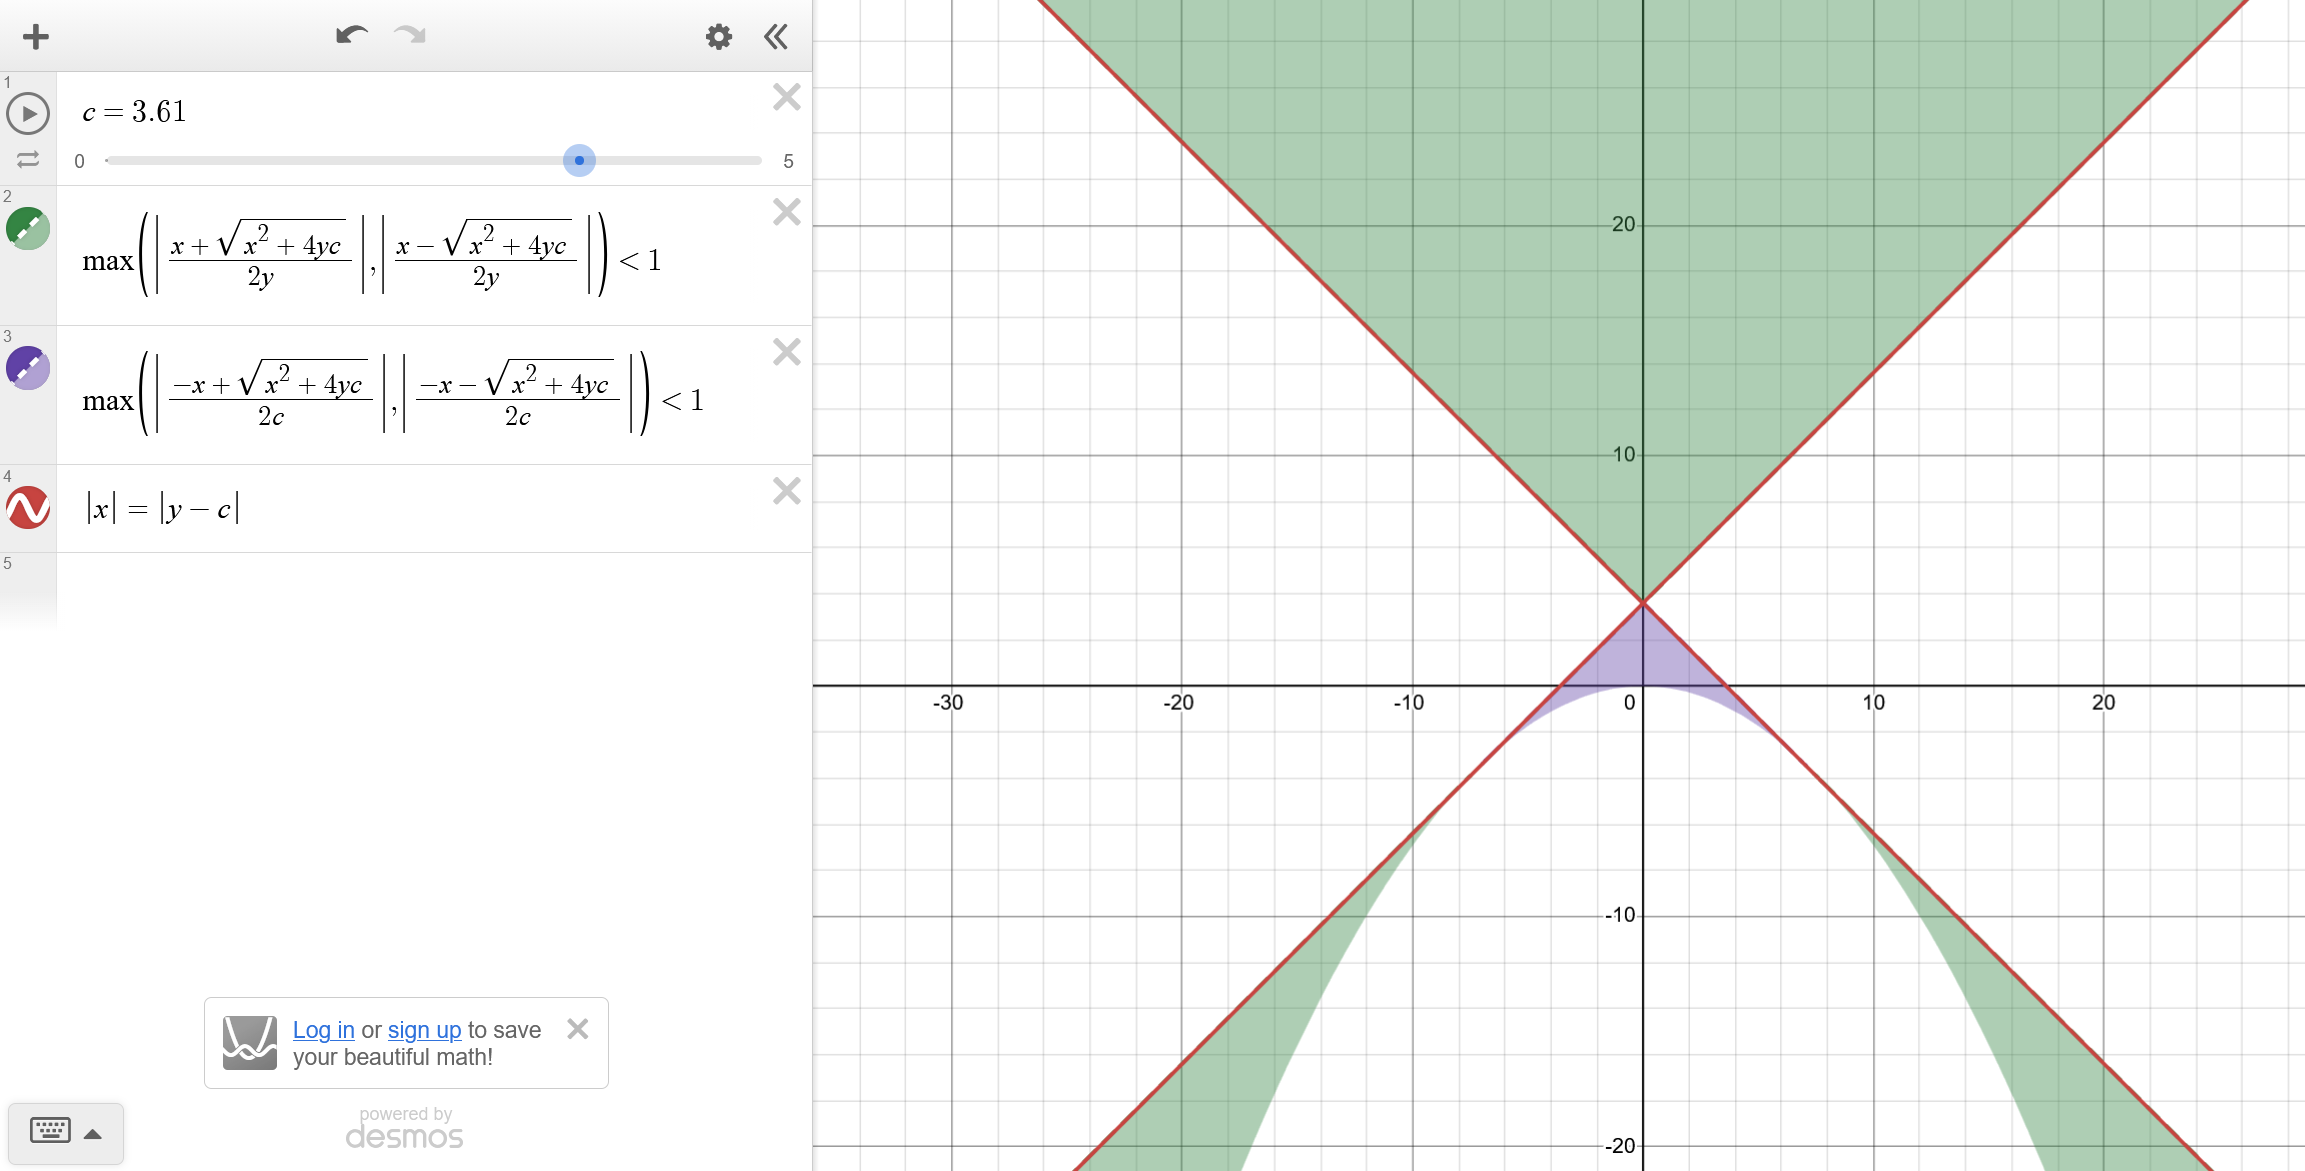
\includegraphics[width=0.8\textwidth]{phase_diagram.png}
    \caption{Phase diagram, or the existence condition of exponentially localized boundary modes.
    Here, $x=\alpha=-\mu$, $y=\beta=w+\Delta$, and the slider $c=\gamma=\Delta-w$.
    Notice how the phase boundary is given by $|x| = |y-c| \Leftrightarrow |\mu|=2|w|$.}
    \label{fig:phase}
\end{figure}

Once we obtain the low-energy eigenvectors $\vec{u}^{(L)}$ and $\vec{u}^{(R)}$,
we label the corresponding Majorana modes:
\[
    b_l = \sum_{j=1}^{2N} u_j^{(L)} c_j,\quad
    b_r = \sum_{j=1}^{2N} u_j^{(R)} c_j.
\]
Because the coefficients are exponentially localized at one of the boundaries,
we also call these the ``boundary modes''.
These approximate boundary operators combine into a single Dirac fermion $a := b_l + ib_r$.
Again, the above sequences $\left\{u_j\right\}$ are not exact eigenvectors of $A$ for finite $N$;
they are approximations for the low-energy modes, should they exist.

Since these boundary operators are not exact zero modes,
the low-energy subspace should obtain a nontrivial effective Hamiltonian.
The only coupling allowed by the $\mathbb{Z}_2$ parity symmetry must have the form
\[
    \Heff = \frac{i}{2} \epsilon b_l b_r = \epsilon \left(
        a^\dagger a - \frac{1}{2}
    \right)
\]
with $\epsilon$ determined by the overlap of the boundary wavefunctions.
Since the coefficient $u_{j}^{(L)}$ decays geometrically away from the left boundary,
and vice versa, the overlap must be proportional to
\[
    \epsilon \sim e^{-N/\xi}\quad \text{with}\quad
    \xi^{-1} \sim -\ln \max \left\{\left|\rho_1\right|, \left|\rho_2\right|\right\},
\]
where $\rho_1$ and $\rho_2$ are the surviving exponential bases.
Again, the splitting is exponentially suppressed in the size of the system,
with degeneracy recovered in the thermodynamic limit.
When $\gamma = 0$, this reduces to
\[
    \xi^{-1} = \ln\left|\frac{\beta}{\alpha}\right|
    = \ln \left|\frac{2w}{\mu}\right|
    = \ln \left|\frac{J_x}{h_z}\right|,
\]
agreeing with the Ising chain correlation length from section~\ref{sec:ising}.
Note that the splitting is not caused by a coupling to the illegal states,
but rather the fact that the boundary operators do not commute exactly with the Hamiltonian:
\[
    [H_{maj}, b_l],\; [H_{maj}, b_r] \sim O\left(e^{-N/\xi}\right).
\]

\subsection{Why are the boundary modes robust?}\label{sec:robust}
The quadratic Hamiltonians discussed in the previous sections are called \emph{noninteracting},
as a product of two fermionic operators is either a site hopping, pair creation, or pair annihilation.
As we have discussed, such a system (assuming matrix $A$ is diagonalizable) splits the Hilbert space
into 2-dimensional sectors with energies $\pm \frac{\epsilon}{2}$,
implying a twofold degeneracy when $\epsilon = 0$.
We also saw how the Kitaev chain yields, under certain circumstances,
boundary modes with exponentially small splitting.

We now argue that this ground sector is robust to local perturbation.
As mentioned in footnote~\ref{foot:parity-super}, the fermionic parity superselection rule
forces any physical operator to contain terms with even number of fermion operators.
The lowest-order parity-preserving operator on the ground sector is $ib_l b_r$,
which necessarily has support on both ends of the wire.
Therefore, any local parity-preserving perturbation must act trivially on the ground sector,
up to corrections by the exponentially small overlap between the left and right boundary modes.

For interacting models, the Hamiltonian consists of higher-order monomials of fermionic operators,
again with even orders.
Such models can be analyzed by slowly turning on the interactions from the noninteracting limit.
If the noninteracting limit shows a topologically protected degenerate ground state,
\emph{and} the rest of the spectrum is gapped away from the ground state throughout the whole process,
then the quasi-adiabatic continuation theorem applies and, as we will see,
the interacting model would also show a similarly degenerate and robust ground sector.

To be specific, consider a continuous deformation $\Tilde{H}(v)$, with $H_0 := \Tilde{H}(v=0)$ noninteracting,
such that the Hamiltonian in question is $H := \Tilde{H}(v=1)$.
Suppose further that $H$ describes a finite chain of fermions
and that $H_0$ maps to a Kitaev chain with boundary modes.
The reference to \textcite{hastings_wen} is basically the following theorem:
\begin{theorem}
    For each local Majorana operator $c_j$, one can find $\Tilde{Y}_j(v)$ such that
    \begin{enumerate}
        \item $\Tilde{Y}_j(v)$ is continuous in $v$,
        \item $\Tilde{Y}_j(v=0) = c_j$, and
        \item $\Tilde{Y}_j(v)$ remains exponentially localized near $j$.
    \end{enumerate}
\end{theorem}
Then, we attach Jordan-Wigner strings to convert the fermionic anticommuting edge operator
into bosonic ones:
\[
    \Tilde{X}_{2j+1} := \Tilde{Y}_{2j+1} \prod_{i=1}^j\left(-ic_{2i-1}c_{2i}\right)\quad \text{and}\quad
    \Tilde{X}_{2j+2} := \Tilde{Y}_{2j+2} \prod_{i=1}^j\left(-ic_{2i-1}c_{2i}\right).
\]
\hwnote{Verify that the Jordan-Wigner strings are meant to survive the adiabatic deformation.}
Applying this construction to the boundary modes $b_l$ and $b_r$, one defines
\[
    \Tilde{X}_l := \sum_{j=1}^{2N} u_j^{(L)} \Tilde{X}_j\quad \text{and}\quad
    \Tilde{X}_r := \sum_{j=1}^{2N} u_j^{(R)} \Tilde{X}_j.
\]
Two observations on these operators:
\begin{enumerate}
    \item $\Tilde{Y}_l$ and $\Tilde{Y}_r$ are still localized near the respective boundaries.
    \item $[\Tilde{H}, \Tilde{X}_{(l, r)}] \approx 0$ and $\left\{P_{maj}, \Tilde{X}_{(l,r)}\right\} = 0$,
        the latter because each term in $\Tilde{X}_{(l, r)}$ consists of an odd number of Majorana operators,
        even if $\Tilde{Y}_{(l,r)}$ consists of higher-order terms.
\end{enumerate}
Thus, algebra generated by $X_{(l,r)}$ and $P_{maj}$ act nontrivially on the adiabatically deformed ground sector,
meaning that $H$ also possesses a nearly-degenerate ground sector.
With two localized operators separated by the chain length,
the previous robustness argument is automatically transferred.

\subsection{Derivation of the phase diagram}\label{sec:phase}
As discussed in section~\ref{sec:quadratic}, the zero modes are physically valid only if $\left\{u_j\right\}$ is square normalizable.
This, in turn, is equivalent to the fact that the eigenvalues of the transfer matrix lying inside the complex unit disc.
This can be efficiently checked using the \emph{Jury stability criterion}:
\begin{theorem}
    The roots of a quadratic polynomial $f(z) = z^2 + az + b\;(a, b \in \mathbb{R})$ lie inside the complex unit disc
    if and only if the following three conditions are met:
    \begin{enumerate}
        \item $f(1) = 1 + a + b > 0$
        \item $f(-1) = 1 - a + b > 0$
        \item $|b| < 1$
    \end{enumerate}
\end{theorem}
\begin{proof}
    Suppose the two roots are $z_1$ and $z_2$.
    Vieta's relations dictate that $z_1 + z_2 = -a,\; z_1 z_2 = b$.
    \begin{enumerate}[label=\roman*)]
        \item Suppose $|z_1|, |z_2| < 1$.
            \begin{enumerate}[label=\arabic*.]
                \item $f(1) = (1 - z_1) (1 - z_2)$ \\
                    If both roots are real, then both factors are positive;
                    if not, $z_2^* = z_1$, so $f(1) = |1-z_1|^2$.
                    In either case, $f(1) > 0$.
                \item $f(-1) = (1 + z_1) (1 + z_2)$ \\
                    Same arguments as the previous case apply.
                \item $|b| = |z_1| |z_2| < 1$
            \end{enumerate}
        \item Suppose the three conditions hold.
            \begin{enumerate}
                \item Suppose $a^2 - 4b < 0$. \\
                    The two roots are complex, and conjugate of each other.
                    Thus, $|z_1| = |z_2| = \sqrt{|b|} < 1$.
                \item Suppose $a^2 - 4b > 0$. \\
                    The two roots are real, so let us arbitrarily order them such that $z_1 \leq z_2$.
                    $f(\pm 1) > 0$ implies that $\pm 1 \notin [z_1, z_2]$.
                    Thus, $z_1, z_2 \in (-1, 1)$.
            \end{enumerate}
    \end{enumerate}
    Thus, the Jury conditions are equivalent to $|z_1|, |z_2| < 1$.
\end{proof}
Take the odd-coefficient transfer matrix.
Its characteristic polynomial is given by $f(z) = z^2 - \frac{\alpha}{\beta}z - \frac{\gamma}{\beta}$,
so assuming $\beta > 0$, the odd coefficients decay away from the left boundary if and only if
$\pm \alpha + \beta - \gamma >0$ and $|\gamma| < |\beta|$.
For the even-coefficient transfer matrix, $f(z) = z^2 + \frac{\alpha}{\gamma}z - \frac{\beta}{\gamma}$,
so the boundary mode exists if and only if $\pm \alpha + \beta - \gamma > 0$ and $|\beta| < |\gamma|$.
Thus, the exact condition for the existence of boundary modes is $|\alpha| < |\beta - \gamma|$ and $|\beta| \neq |\gamma|$,
or in the SPSC language, $|\mu| < 2|w|$ and $w, \Delta \neq 0$. \qed

\subsection{Bulk spectrum under periodic boundary conditions}
Suppose we endow the SPSC chain with periodic boundaries,
or more generally, we consider a region sufficiently far from the boundaries
such that the edge effects can be neglected:
\[
    H_F = \sum_{j=1}^N \left(
        - w \left( a_j^\dagger a_{j+1} + a_{j+1}^\dagger a_j \right)
        + \Delta \left( a_j a_{j+1} + a_{j+1}^\dagger a_j^\dagger \right)
        - \mu \left( a_j^\dagger a_j - \frac{1}{2} \right)
    \right)\quad
    (a_{N+1} := a_1).
\]
Here, the system respects translational symmetry, so the momentum basis is useful:
\[
    a_k := \frac{1}{\sqrt{N}} \sum_{j=1}^N a_j e^{-ikja}\quad
    \left(ka = -\pi, -\frac{N-2}{N}\pi, \cdots, \frac{N-2}{N}\pi, \pi\right),
\]
where $a$ is the lattice spacing.
Straightforward Fourier transform yields:
\[
    H_F = -\sum_k \begin{pmatrix}
        a_k^\dagger & a_{-k}
    \end{pmatrix} \begin{pmatrix}
        w\cos ka + \frac{\mu}{2} & -i\Delta\sin ka \\
        i\Delta\sin ka & -\left(w\cos ka + \frac{\mu}{2}\right)
    \end{pmatrix} \begin{pmatrix}
        a_k \\ a_{-k}^\dagger
    \end{pmatrix}.
\]
We thus introduce the \emph{Nambu spinor} $\Psi_k := \begin{pmatrix} a_k \\ a_{-k}^\dagger \end{pmatrix}$
and the momentum-dependent \emph{Bogoliubov-de Gennes} Hamiltonian $\mathcal{H}(k)$ to write
\[
    H_F = -\sum_k \Psi_k^\dagger \mathcal{H}(k) \Psi_k.
\]
The Nambu spinor is a useful object because the momentum is conserved while the particle number is not;
since $a_k$ annihilates a particle with momentum $k$ while $a_{-k}^\dagger$ creates one with momentum $-k$,
both operators act to decrease the total momentum by $k$.
Conversely, both operators in $\Psi_k^\dagger$ increase the total momentum by $k$.

Diagonalizing $\mathcal{H}(k)$, one naturally discovers the \emph{Bogoliubov transformation}:
\[
    \begin{pmatrix}
        \eta_k \\ \eta_{-k}^\dagger
    \end{pmatrix} = \begin{pmatrix}
        u_k & -iv_k \\ iv_k & u_k
    \end{pmatrix} \begin{pmatrix}
        a_k \\ a_{-k}^\dagger
    \end{pmatrix}\quad (u_k, v_k \in \mathbb{R}, u_k^2 + v_k^2 = 1).
\]
The form of the matrix and the conditions of $u_k, v_k$ are such that
$\eta_k$ satisfies the anticommutation relations.
If $\begin{pmatrix} u_k \\ iv_k \end{pmatrix}$ and $\begin{pmatrix} -iv_k \\ u_k \end{pmatrix}$
are the unit eigenvectors with respective eigenvalues
\[
    \mp E(k) := \mp \sqrt{w^2 + \left(\frac{\mu}{2}\right)^2+w\mu\cos ka},
\]
then the Hamiltonian reduces to
\[
    H_F = \sum_k E(k) \left(\eta_k^\dagger\eta_k - \eta_{-k}\eta_{-k}^\dagger\right)
    = \sum_k E(k) \left(\eta_k^\dagger\eta_k + \eta_{-k}^\dagger\eta_{-k} - 1\right)
    = \sum_k E(k) \left(\eta_k^\dagger\eta_k - \frac{1}{2}\right).
\]
Thus, $E(k)$ is the exact dispersion relation of the Kitaev chain,
with the ground state $\ket{G}$ satisfying $\forall k.\; \eta_k\ket{G} = 0$.

For the special point $\Delta = w$, this reduces to
\[
    E(k) = \pm\sqrt{w^2 + \left(\frac{\mu}{2}\right)^2+w\mu\cos ka}.
\]
Depending on the sign of $w\mu$, the minimum energy gap is found at either $ka = 0$ or $\pi$,
such that the energy gap evaluates to $\left|\left|w\right|-\left|\frac{\mu}{2}\right|\right|$.
Thus, the energy gap closes exactly at the phase boundary $|\mu| = 2|w|$.
In the general case, the energy gap loses precisely when both squared terms vanish,
the $\Delta\sin ka$ term imposing $ka = 0$ or $\pi$.
Thus, assuming $\Delta > 0$, the energy gap vanishes precisely when $|\mu| = 2|w|$.

Finally, let us calculate the two-point correlator
\[
    C(r) := \braket{a_j^\dagger a_{j+r}}
    = \frac{1}{N} \sum_{kq} \braket{a_k^\dagger a_q} e^{ikja} e^{-iq(j+r)a}.
\]
Then, the inverse Bogoliubov transformation yields
\[
    a_k^\dagger = iv_k\eta_k + u_k\eta_{-k}^\dagger,\quad
    a_q = u_q\eta_{-q} - iv_q\eta_q^\dagger
\]
\[
    \implies \braket{a_k^\dagger a_q}
    = v_k v_q \braket{G | \eta_k \eta_q^\dagger | G}
    = v_k^2 \delta_{kq}
\]
\[
    \implies C(r) = \frac{1}{N}\sum_k v_k^2 e^{-ikra}.
\]
Calculating the eigenvector of $\mathcal{H}(k)$, one finds that
\[
    v_k^2 = \frac{1}{2} \left(1 - \frac{\zeta(k)}{E(k)}\right)\quad
    \left(\zeta(k) := w\cos ka + \frac{\mu}{2}\right)
\]
\begin{align*}
    \implies C(r)
    &= \frac{1}{N} \sum_k \frac{1}{2}\left(1 - \frac{\zeta(k)}{E(k)}\right) e^{-ikra} \\
    &\xrightarrow{N\rightarrow\infty} \frac{a}{2\pi}
        \int_{-\pi/a}^{\pi/a} dk \frac{1}{2}\left(1 - \frac{\zeta(k)}{E(k)}\right) e^{-ikra} \\
    &= \frac{1}{2} \left(
        \delta_{r,0} - \frac{a}{2\pi}\int_{-\pi/a}^{\pi/a} dk \frac{w\cos ka + \frac{\mu}{2}}{
            \sqrt{\left(w\cos ka + \frac{\mu}{2}\right)^2 + \Delta^2\sin^2 ka}
        }
    \right).
\end{align*}

In the case $\Delta = w$ and $r > 0$, the two-point function evaluates to
\begin{align*}
    C(r)
    &= -\frac{a}{4\pi}\int_{-\pi/a}^{\pi/a} dk \frac{w\cos ka + \frac{\mu}{2}}{\sqrt{
        \left(\frac{\mu}{2}\right)^2 + \mu w \cos ka + w^2
    }} \\
    &= -\frac{a}{4\pi} \oint_{|z|=1} \frac{dz}{iaz} \frac{\frac{w}{2}\left(z+z^{-1}\right)+\frac{\mu}{2}}{
        \sqrt{\left(\frac{\mu}{2}\right)^2 + w^2 + \frac{\mu w}{2} \left(z+z^{-1}\right)}
    } z^{-r} & (z := e^{ika}) \\
    &= \frac{i}{16\pi}\sqrt{\frac{w}{2\mu}} \oint_{|z|=1} dz z^{-\left(r + \frac{3}{2}\right)}
        \frac{z^2 + \frac{\mu}{w}z + 1}{\sqrt{\left(z+\frac{\mu}{2w}\right)\left(z+\frac{2w}{\mu}\right)}}.
\end{align*}
The zeros of the radicand are $-\frac{\mu}{2w}$ and $-\frac{2w}{\mu}$,
which lie on the unit circle exactly on the phase boundary $|\mu| = 2|w|$.
\hwnote{TODO: Extract the asymptotic form $C(r) \sim e^{-r/\xi}$ to verify that the correlation length $\xi$
agrees with the previous methods.}

\subsection{Topological invariant}\label{sec:invar}
In section~\ref{sec:robust}, we argued for the robustness of boundary modes under adiabatic deformations
of the Hamiltonian, possibly including higher-order interaction terms,
so long as the bulk gap does not close.
This would imply that the phase diagram also deforms adiabatically.
In this sense, the phase of the Kitaev chain is \emph{topological}, i.e., it survives
every possible adiabatic deformation that leaves the energy gap open.
This leaves one wondering,
"How can I tell if two Hamiltonians are showing the same(=adiabatically connected) phase?"
One answer is to assign a number $\nu$ to each phase, satisfying the following conditions:
\begin{enumerate}
    \item $\nu(H)$ is a function of the Hamiltonian only.
    \item Along a continuous path $H(v)\; (v\in[0,1])$ where the bulk gap does not close,
        $\nu(H(v))$ is also continuous.
    \item $\nu$ can take only discrete values.
\end{enumerate}
Notice how the last two points imply that \emph{on each connected component
of the space of gapped Hamiltonians in consideration,
$\nu$ takes distinct discrete values.}
This allows us to classify phases in an intrinsic manner robust to adiabatic deformations!
Such a number is called a \emph{topological invariant} of the system.

So, how do we find such a number $\nu$?
Suppose we rewrite the momentum-dependent Hamiltonian as
\[
    \mathcal{H}(k) := \vec{d}(k) \cdot \vec{\tau},\quad \text{where}\quad
    \vec{\tau} = \begin{pmatrix}
        \tau^x & \tau^y & \tau^z
    \end{pmatrix}.
\]
Effectively, $\vec{d}(k)$ is a 3D parametrization of the $2\times2$ traceless Hermitian matrices.
For the Kitaev chain, this is given by
\[
    \vec{d}(k) = \begin{pmatrix}
        0 & \Delta\sin ka & w\cos ka + \frac{\mu}{2}
    \end{pmatrix},
\]
residing in the $yz$ plane.
Notice that on this plane, the gapless Hamiltonian is reached only at the origin.
With all of this work, we have reduced the task of finding a topological invariant of the Kitaev chain
to that of classifying all loops in $\mathbb{R}^2 \setminus \left\{0\right\}$.
From basic algebraic topology (apparently), one natural classification is the \emph{winding number}
of the curve around the origin.
It is a discrete, homotopy-invariant number of the curve $\vec{d}(k)$.
Since there are only two phases in our case, one might expect that the winding number mod 2 would be relevant.
(See also section~\ref{sec:ptcl_hole} for why $\nu \in \mathbb{Z}_2$.)

Assuming the previous argument holds, when does the curve $\vec{d}(k)$ wind around the origin?
The curve passes through the $z$ axis ($y=0$) at exactly $ka = 0, \pi$,
so if $d_z(0)$ and $d_z(\pi/a)$ have the same sign, the curve must wind the origin an even number of times;
if different, an odd number of times.
Thus, $\nu := \mathrm{sign}\left(d_z(0) d_z\left(\frac{\pi}{a}\right)\right)$ classifies all curves in this way.
When $|\mu| \neq 2|w|$, the product does not vanish and $\nu$ is well-defined.
In fact, explicit calculation yields $\nu = \mathrm{sign}\left(\left(\frac{\mu}{4}\right)^2 - w^2\right)$,
so the boundary modes exist precisely when $\nu = -1$.
Thus, this definition of $\nu$ correctly distinguishes the topological and trivial phases of the Kitaev chain.

To express this in terms of the Hamiltonian itself, we introduce the Majorana formalism again.
Notice that
\[
    c_{2j-1} = a_j + a_j^\dagger = \frac{1}{\sqrt{N}}\sum_k \left(a_k+a_{-k}^\dagger\right)e^{-ikja}\quad
    \text{and}\quad
    c_{2j} = i\left(a_j^\dagger - a_j\right) = \frac{1}{\sqrt{N}}\sum_k \left(
        i\left(a_{-k}^\dagger - a_k\right)
    \right) e^{-ikja}.
\]
Thus, we define the momentum Majorana operators
$c_k := a_k + a_{-k}^\dagger$ and $c_k' = i\left(a_{-k}^\dagger - a_k\right)$.
The Nambu spinors are then expressed as
\[
    \Psi_k = \begin{pmatrix}
        a_k \\ a_{-k}^\dagger
    \end{pmatrix} = \begin{pmatrix}
        \frac{c_k + ic_k'}{2} \\ \frac{c_k - ic_k'}{2}
    \end{pmatrix} = \begin{pmatrix}
        \frac{1}{2} & \frac{i}{2} \\ \frac{1}{2} & -\frac{i}{2}
    \end{pmatrix} \begin{pmatrix}
        c_k \\ c_k'
    \end{pmatrix} := U\Gamma_k.
\]
Note that $\Gamma_k^\dagger = \Gamma_{-k}^T$. Hence,
\[
    H_F = -\sum_k \Gamma_k^\dagger U^\dagger \mathcal{H}(k) U\Gamma_k
    = -\sum_k \frac{i}{2} \Gamma_{-k}^T \begin{pmatrix}
        0 & w\cos ka + \frac{\mu}{2} +i\Delta\sin ka \\
        -\left(w\cos ka + \frac{\mu}{2}\right) + i\Delta\sin ka & 0
    \end{pmatrix} \Gamma_k
\]
The matrix $A(k) := -2iU^\dagger \mathcal{H}(k) U$ is Hermitian skew-symmetric,
i.e., $A(k)^\dagger = -A(k)$.
The imaginary parts of the elements vanish at precisely $ka=0, \pi$,
at which points $A$ is real skew-antisymmetric and the Pfaffian well-defined.
In fact, $\pfaff A(0) = d_z(0)$ and $\pfaff A(\pi/a) = d_z(\pi/a)$, so we find the celebrated expression
\[
    \nu = \mathrm{sign}\left(\pfaff A(0) \cdot \pfaff A\left(\frac{\pi}{a}\right)\right).
\]

We note one particular consequence of this invariant.
\begin{theorem}
    The bulk topological invariant $\nu = -1$ if and only if, under open boundary conditions,
    there exist exponentially localized edge modes.
\end{theorem}
This is significant, because the existence of boundary modes can be inferred
using only properties of the bulk!
This concept is called the \emph{bulk-boundary correspondence},
wherein the topology of the bulk Hamiltonian maps to the physics near the boundary of the system.
This concept can be stated and proven in more generality, for example using $K$-theory and index theory.

\subsection{Particle-hole symmetry}\label{sec:ptcl_hole}
Certain symmetries constrain the type of Hamiltonians $\mathcal{H}(k)$,
one of which is the so-called \emph{particle-hole symmetry} (or \emph{charge conjugation} in some cases).\footnote{%
It should be noted that the concept of particle-hole symmetry is used confusingly across multiple areas of physics.~\cite{zirnbauer_ptcl_hole}
To avoid any confusion, we only define it in terms of the Bogoliubov-de Gennes Hamiltonian.
}
The symmetry action is characterized by the antiunitary transformation $\Psi_k \mapsto \tau^x \Psi_k^\dagger$
mapping every quasiparticle excitation energy $E$ to one of energy $-E$.
Equivalently,
\[
	\tau^x \mathcal{H}(k)^* \tau^x = -\mathcal{H}(-k).
\]
Using the complex conjugation operator $K$ to define the antiunitary operator $\Theta := \tau^x K$,
the condition can be expressed as
\[
	\Theta \mathcal{H}(k) \Theta^{-1} = -\mathcal{H}(-k).
\]

The primary consequence of the particle-hole symmetry is the symmetric energy bands.
If $\mathcal{H}(k)\ket{u(k)} = E(k)\ket{u(k)}$, then because $E(k) \in \mathbb{R}$,
\[
	\mathcal{H}(-k)\Theta\ket{u(k)} = -\Theta\mathcal{H}(k)\ket{u(k)} = -\Theta E(k)\ket{u(k)} = -E(k)\ket{u(k)}.
\]
Thus, $E(-k) = -E(k)$, or for each band $E(k)$, there is a corresponding band $-E(-k)$.

For a general $\mathcal{H}(k) = \vec{d}(k) \cdot \vec{\tau}$, this symmetry is equivalent to the constraint
\[
	d_x(-k) = -d_x(k),\quad d_y(-k) = -d_y(k)\quad \text{and}\quad d_z(-k) = d_z(k).
\]
For the family of maps $S^1 \rightarrow \mathbb{R}^3\setminus\{0\}$ satisfying this property, there are two connected components.
In our case, two curves are path-connected precisely when they are homotopic,
that is, continuously deformed from one to another.
The topological invariant $\nu$ calculated in section~\ref{sec:invar} is a complete homotopic invariant of this space.\footnote{%
This also explains why only $k=0$ and $\pi/a$ are used to define $\nu$:
they are the fixed points of the involution $k \mapsto -k$!
}

Let us state this more rigorously.
A $d$-dimensional free-fermion system with translational symmetry can be characterized
by the Bogoliubov-de Gennes Hamiltonian $\mathcal{H}(k)$.
Here, $k$ lies in the $d$-dimensional Brillouin zone, homeomorphic to the $d$-dimensional torus $T^d$.
We will only consider gapped Hamiltonians, so let $F$ denote the space of such Hamiltonians.
For the Kitaev chain, the Brillouin zone is identified with the circle ($T^1 =  S^1$),
while the space of $2\times 2$ Hamiltonians (up to constant shifts) is naturally homeomorphic to $\mathbb{R}^3\setminus\{0\}$.
(Here, $\cong$ signifies homeomorphism.)
The classification of such Hamiltonians, or the topological phases,
is thus the study of connected components of the family of such maps.

In general, we denote as $[X,Y]$ the homotopic classes of continuous maps $f: X \rightarrow Y$.
However, we are currently imposing certain conditions on the maps.
A general method is to define a group $G$ with homeomorphic representations
\[
	\rho_X: G \rightarrow \mathrm{Homeo}(X)\quad \text{and} \rho_Y: G \rightarrow \mathrm{Homeo}(Y).
\]
We thus impose that these actions must be preserved:
\[
	\forall g \in G,\; x \in X.\; f(\rho_X(g)(x)) = \rho_Y(g)(f(x)).
\]
Such maps are called \emph{equivariant}, and the homotopic classes of them the \emph{equivariant homotopy} $[X,Y]_G$.
(Note that despite the notation, the equivariant homotopy depends on the chose group actions on both $X$ and $Y$,
not just on the abstract group $G$.)
In our case, the relevant equivariant homotopy is $[T^d, S^2]_{\mathbb{Z}_2}$,
where $\mathbb{R}^3\setminus\{0\} \simeq S^2$ (homotopy) and can be replaced,
while $\mathbb{Z}_2$ acts such that $\rho_X(-1)(k) = -k$ and $\rho_Y(-1)_(x, y, z) = (-x, -y, z)$.
With this, one can calculate $[S^1, S^2]_{\mathbb{Z}_2} \cong \mathbb{Z}_2$,
which would predict two distinct phases, just as we have calculated.\footnote{%
For more complicated models, the so-called \emph{classifying space} $F$ is defined differently,
possibly containing Hamiltonians of different dimensions.
To accomodate all such microscopic details, one defines two Hamiltonians to be equivalent
if they differ only by trivial bands:
\[
	\mathcal{H}_1 \sim_{st} \mathcal{H}_2 \iff \mathcal{H}_1 \oplus \mathcal{E}_1 \simeq \mathcal{H}_2 \oplus \mathcal{E}_2,
\]
where $\mathcal{E}$ denotes Hamiltonians with only trivial bands.
Let $\mathscr{H}_n$ denote the $n$-dimensional gapped Hamiltonians.
One defines a natural inclusion map $\iota_n: \mathscr{H}_n \hookrightarrow \mathscr{H}_{n+1}$ by
\[
	\iota_n(\mathcal{H}) := \mathcal{H} \oplus \begin{pmatrix} 1 & 0 \\ 0 & -1 \end{pmatrix},
\]
thus defining an increasing chain
\[
	\mathscr{H}_1 \hookrightarrow \mathscr{H}_2 \hookrightarrow \mathscr{H}_3 \hookrightarrow \cdots.
\]

So, to be precise, the relevant topology is $[T^d, F]$, where $F$ denotes the stable limit of this chain,
together with the appropriate symmetry constraints.
The \emph{Bott periodicity theorem} states that there are exactly 8 distinct real Bott spaces $R_q$
and 2 distinct complex Bott spaces $C_q$,
(Apparently, one has $\Tilde{KO}^{-q}(S^d) \cong \pi_0(R_{q-d})$,
allowing one to classify phases only using the connected components of these ten Bott spaces.
\hwnote{What?})
In fact, only three discrete symmetries --- time reversal, particle-hole, and chirality --- are sufficient
to completely determine which Bott space is relevant to the given physical system.
This is called the \emph{Altland-Zirnbauer classification}, of which the Kitaev chain belongs to class D.
}

Consequently, the classification is largely independent of the microscopic realization.
Once the system admits a Bogoliubov-de Gennes description with the prescribed symmetry class,
its topological phase depends only on the corresponding equivariant homotopy class,
rather than on microscopic quantities such as lattice geometry, hopping amplitudes, or the number of trivial bands.

\printbibliography
\end{document}

